\section{Support Vector Machine and Structured Learning}

\begin{frame}{Structured Problems}
    \begin{itemize}
          \item Do not predict single value, but a structured object,
        \begin{itemize}
              \item[] \eg predict a path
        \end{itemize}
          \item Utilize structured loss for a better evaluation of prediction, 
        \begin{itemize}
              \item[] \eg quantize prediction error for tracking based on a tree comparison of lineages
        \end{itemize}
    \end{itemize}
\end{frame}


\begin{frame}{Structured Problem - Examples}
    \begin{figure}
        \centering
        \begin{subfigure}[b]{0.4\textwidth}
            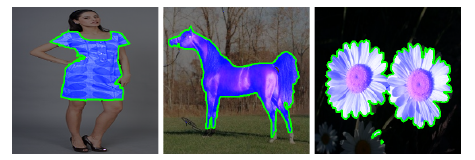
\includegraphics[width=\textwidth]{images/external/bertelli.png}
            \caption{Segmentation}
            \label{fig:bertelli}
        \end{subfigure}%
        \begin{subfigure}[b]{0.4\textwidth}
            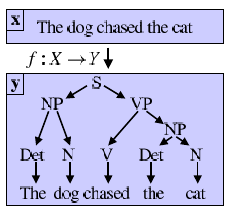
\includegraphics[width=\textwidth]{images/external/joachims-struct-svm-example.png}
            \caption{Language Parse Tree}
            \label{fig:joachims}
        \end{subfigure}
        \caption{(\protect\subref{fig:bertelli})\footcite{bertelli_11_kernelized}, (\protect\subref{fig:joachims})\footcite{joachims_04_support}}
    \end{figure}
\end{frame}


\begin{frame}{Support Vector Machines - Prediction}
    \begin{itemize}
          \item linear two-class classifier
          \item score input $\textbf{x}$ and assign label according to sign of score
        \begin{itemize}
              \item[] $y_{\text{predict}} = \sgn\left(\textbf{w}^{\intercal}\textbf{x} + b\right)$
        \end{itemize}
          \item parameters $\textbf{w}$, $b$ determined by training
    \end{itemize}
\end{frame}


\begin{frame}
    \frametitle{Support Vector Machines - Training }
    \begin{itemize}
          \item minimize regularized cost function
          \item[] \begin{align}
            &\textbf{w}^*, b^*, \xi^*  = \argmin_{\textbf{w}, b, \xi} \frac{1}{2} \textbf{w}^{\intercal} \textbf{w}
            + \frac{C}{kN}\sum_{n=1}^N\left(\xi_n\right)^k \\
            &\phantom{\textbf{w}^*, b^*, \xi^*  = }\st \nonumber \\ 
            &y_n\left(\textbf{w}^\intercal\textbf{w}+b\right) \geq 1 - \xi_n \; \forall n \in \{l \in
            \mathbb{N} | l < N\}
        \end{align}
          \item typically, $k\in\{1,2\}$
        \item \fullcite{barber_12_bayesian} for more details
    \end{itemize}
\end{frame}


\begin{frame}
    \frametitle{Support Vector Machines - Two Class Example}
    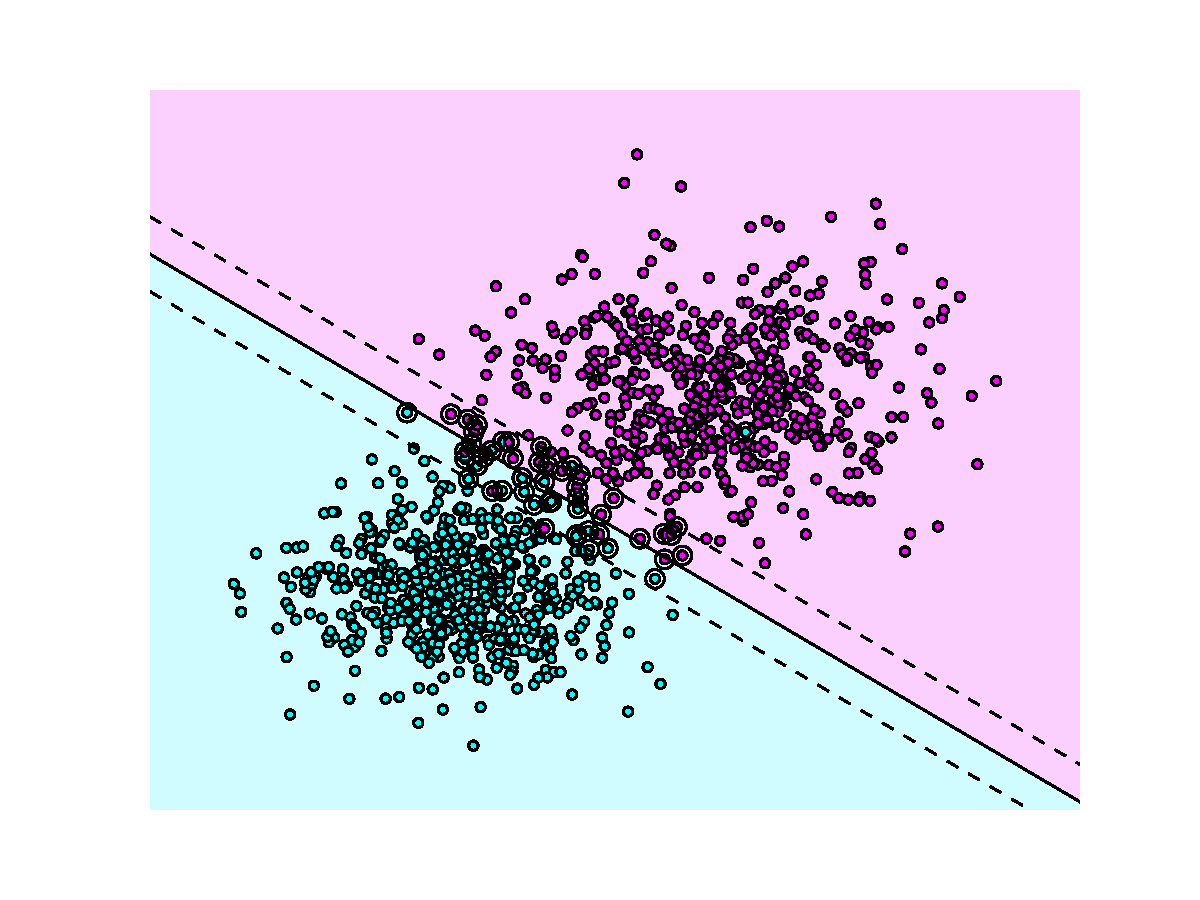
\includegraphics[width=\textwidth]{images/two_class_svm.pdf}
\end{frame}


\begin{frame}
    \frametitle{From Single/Two Class to Multi Class}
    \begin{itemize}
          \item Introduce one SVM classifier ($\textbf{w}_y, b_y$) for each class $y$
          \item For prediction, the maximum scoring classifier determines the label
        \begin{itemize}
              \item[] $\displaystyle y_{\text{predict}} = \argmax_y \;
            \bigl(\left(\textbf{w}_y\right)^{\intercal}\textbf{x} + b_y\bigr) $
        \end{itemize}
    \end{itemize}
\end{frame}


\begin{frame}
    \frametitle{Support Vector Machines - Three Class Example}
    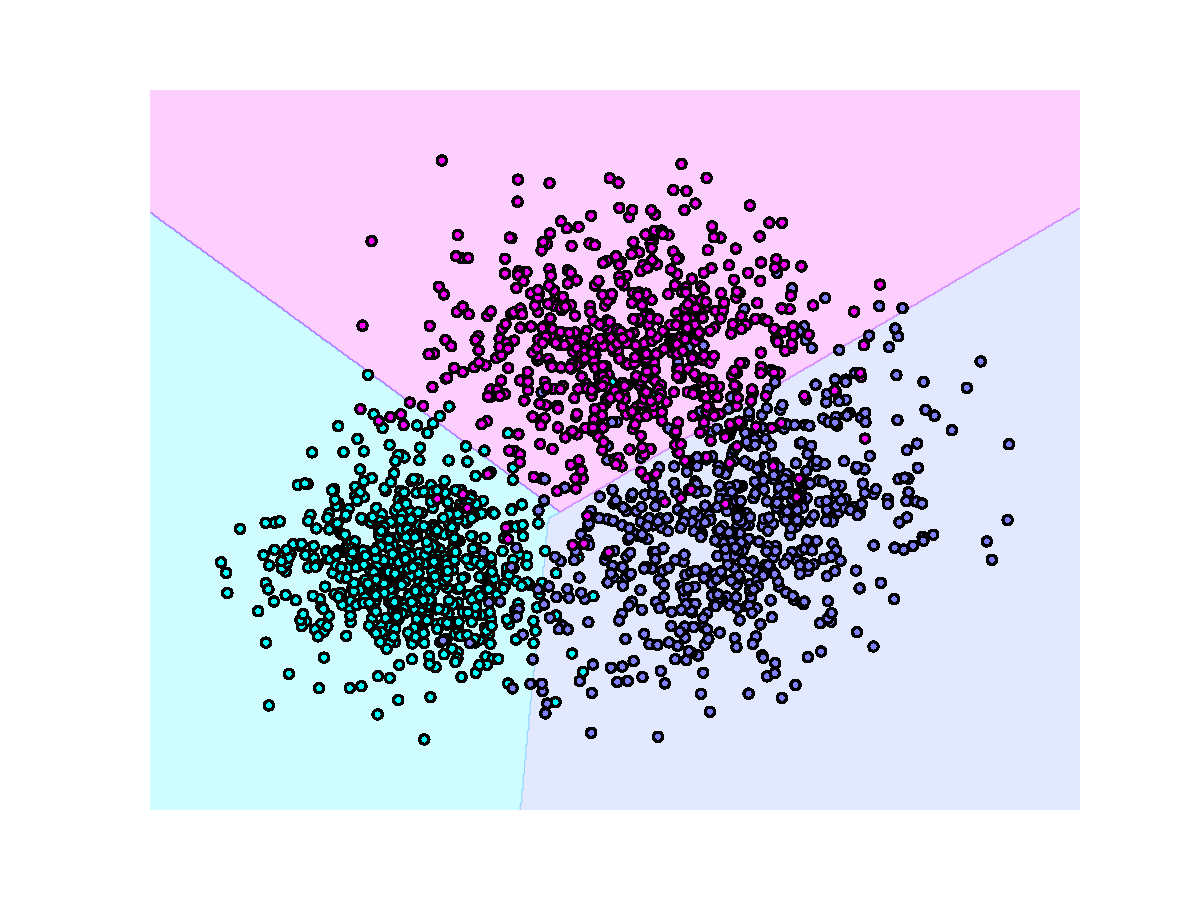
\includegraphics[width=\textwidth]{images/three_class_svm.pdf}
\end{frame}

\begin{frame}
    \frametitle{From SVM to Structured Learning}
    \begin{itemize}
          \item Generalize score: $\svmScore \rightarrow F(\VEC{x}, Y; \VEC{w})$, $Y \in
        \mathcal{Y}$ structured
          % \item Reasonable choice: $\structSvmScore = \linearScore$%\combinedFeature$
          \item Prediction: $\displaystyle Y_{\text{predict}} = \argmax_Y\ \structSvmScore $%= \argmax_Y \linearScore$
          \item In General: $|\mathcal{Y}| = \infty$
        \begin{itemize}
              \item[$\Rightarrow$] Choose $F$ appropriately, \eg $F=\linearScore$
        \end{itemize}
          \item[] \cf \fullcite{joachims_04_support}
    \end{itemize}
\end{frame}


\begin{frame}
    \frametitle{Structured SVM Training}
    \begin{itemize}
          \item Introduce structured loss $\structuredLoss$, \eg Hamming loss
          \item Minimize loss and ``push away'' training data from wrong examples
          \item[]
        \begin{align}
            &\min_{\VEC{w}, \xi} \frac{1}{2}\dualvec{w}\VEC{w} + \frac{C}{kN} \sum_{i=1}^N(\xi_i)^k
            \\ \nonumber
            &\phantom{\min_{\VEC{w}, \xi}} \st \\ \nonumber
            &F(\VEC{x}_i, Y_i) - F(\VEC{x}_i, Y) \ge \Delta(Y, Y_i) - \xi_i \; \; \forall i, \; \forall Y \in \mathcal{Y}\setminus Y_i 
        \end{align}
          \item Infinite number of constraints.
    \end{itemize}

\end{frame}

\begin{frame}
    \frametitle{Structured SVM Training}
    \begin{itemize}
          \item Iteratively add ``most violated constraints''
          \item[]
        \begin{align}
            &\min_{\VEC{w}, \xi} \frac{1}{2}\dualvec{w}\VEC{w} + \frac{C}{kN} \sum_{i=1}^N(\xi_i)^k
            \\ \nonumber
            &\phantom{\min_{\VEC{w}, \xi}} \st \\ \nonumber
            &\max_{Y\in\mathcal{Y}} \bigl(\Delta(Y, Y_i) + F( \VEC{x}_i, Y) - F(\VEC{x}_i, Y_i) \bigr) \le \xi_i
            \; \forall i 
        \end{align}
        \begin{itemize}
              \item[$\Rightarrow$] At each iteration solve a potentially expensive problem:
              \item[] $\displaystyle \max_{Y\in\mathcal{Y}\setminus Y_i} \bigl(\Delta(Y, Y_i) + F( \VEC{x}_i, Y) \bigr)$
        \end{itemize}
    \end{itemize}
    
\end{frame}

%%% Local Variables: 
%%% mode: latex
%%% TeX-master: "../main"
%%% End: 
